\subsection{Porter's Five Forces}

Using Porter's Five Forces, we can analyse the market, and how it affects our product. As we deem the market dangerous, as it is occupied a lot, we believe this business model can be useful for the process. Figure \ref{fig:five_forces} is a visual representation of the model, where our considerations are pointed out for the forces. Each of these will be further explained.

\begin{figure}[h]
    \begin{center}
        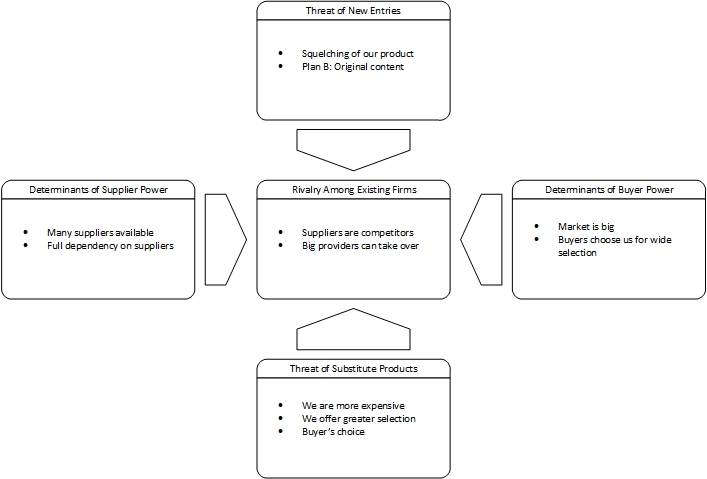
\includegraphics[scale=0.65]{./pics/five_forces}
        \caption{Porter's Five Forces for the project}
        \label{fig:five_forces}
    \end{center}
\end{figure}

\subsubsection*{Determinants of Supplier Power}
The suppliers for the project are providers of motion pictures through streaming over the internet. There are many of these providers, which is the main reasoning for the project. For the project to succeed, these providers must agree to supply the project. This causes a thread, as we then become very dependent on the suppliers. There also exists the thread of the suppliers becoming too big, challenging our idea.

\subsubsection*{Determinants of Buyer Power}
As there already exists providers for motion pictures through streaming that are thriving, it can be concluded that the market exists, but is risky to enter. Our product differs in our wide range of selection, as we serve as a gateway to the existing companies, and do not quelch the existing market. The hope is that users will choose us for this quality, and that we can capture the part of the market that want to use several services, but don't want to pay for them all.

\subsubsection*{Thread of Substitute Products}
The services that exist for the market are not combining the effort of all suppliers, which gives us both an advantage and a disadvantage: As we are a gateway to existing services, we offer a greater selection, but we are therefore also more expensive. The greatest thread of a substitute is if an existing provider expands to the point that we are not needed as a service.

\subsubsection*{Thread of New Entries}
If a new competitor is to enter the market, a possible outcome is loss of suppliers. Imagine this scenario: The new competitor will gain suppliers, possibly by focusing on our product's weak points, and perhaps gain some of our suppliers as well. As there is a risk involving loss of suppliers, a natural backup plan would be to create media of original content. If our suppliers are then lost, we will simply become another streaming service. To avoid this, we must focus on our weaknesses, and make sure we are never seen as the second best choice for suppliers.

\subsubsection*{Rivalry Among Existing Firms}
One of the problems in this business is the fact that the suppliers can be seen as competitors. They are suppliers, but they are not dependent on us, although we are completely dependent on them in the start. The greatest streaming services are very successful in themselves, and if they become too big, we are not needed as a service.

\subsubsection*{Discussion}
The market itself is greatly occupied, which is both positive and negative. On one hand, we might be an unnecessary service. On the other hand, we offer a collection of the existing services, for ease of access and saving of money. The dependency on our suppliers is a risk, as we can only succeed in this project if a set of providers agree to supply access. The market itself is therefore a difficult one, as we twist it to our advantage, but at a great risk.